% Wczytanie szablonu
\documentclass[nostrict]{Szablon}

% Definicja dokumentu
\usepackage[unicode=true]{hyperref}
\usepackage{listings}
\newcommand\PDFtitle{Tytuł pracy}
\newcommand\PDFauthors{Imie Nazwisko}
\hypersetup{
  pdftitle={\PDFtitle},
  pdfauthor={\PDFauthors},
}

% Zmiana czcionki dla symulacji maszynopisu (verbatim)
\makeatletter
\renewcommand{\verbatim@font}{\ttfamily\small}
\makeatother

% Część właściwa pracy
\begin{document}
\chapter*{Streszczenie}
\addcontentsline{toc}{chapter}{Streszczenie}  

\chapter*{Abstract}
\addcontentsline{toc}{chapter}{Abstract}  

\chapter*{Spis treści}
\addcontentsline{toc}{chapter}{Spis treści}

\tableofcontents

\chapter*{Wykaz ważniejszych oznaczeń i skrótów}
\addcontentsline{toc}{chapter}{Wykaz ważniejszych oznaczeń i skrótów}


\section{Organizacja (Bartosz Strzelecki)}\label{s:org}
W tym podrozdziale przedstawiono harmonogram prac, wraz z ich przewidywanym terminem realizacji.
Ponadto zaprezentowano skład zespołu projektowego, kompetencje ich członków oraz podział zadań.
\subsection{Główne etapy projektu}
\begin{center}
  \begin{tabular}{| m{30em} | m{12em}|} 
  \hline
  Etap & Termin realizacji \\
  \hline\hline
  Wybór i analiza konkretnego kontekstu historycznego. & Kwiecień 2023 \\
  \hline
  Syntetyczny opis modelu postrzegania przestrzeni na podstawie dzieł pisanych, architektury i sztuki. & Kwiecień — Maj 2023 \\
  \hline
  Przegląd rozwiązań stosowanych w grach strategicznych z wybranego okresu oraz dodatkowo mechanizmów z innych gier, które mogłyby być zaadoptowane na potrzeby projektu. & 2, 3 kwartał 2023 \\
  \hline
  Opracowanie fabuły, selekcja postaci i wydarzeń, a także określenie zakresu autonomii świata gry oraz możliwości modyfikowania go przez gracza. & Czerwiec 2023 \\
  \hline
  Opracowanie szczegółowej koncepcji i projektu gry, w tym projekt mechanizmów zawartych w prototypie. & Lipiec 2023 \\
  \hline
  Implementacja poszczególnych funkcjonalności gry. & 4 kwartał 2023 \\ 
  \hline
  Testowanie, weryfikacja założeń i walidacja. & Listopad — Grudzień 2023 \\
  \hline
  Stworzenie dokumentacji przeprowadzonych prac. & 3, 4 kwartał 2023 \\
  \hline
\end{tabular}
\end{center}
Przewidywany termin zakończenia prac nad projektem to grudzień 2023 roku.
\begin{figure}[htbp]
    \centering
    \includegraphics[width=1\textwidth]{uml/Harmonogram}
    \caption{Harmonogram przedstawiony w postaci diagramu gantt.}
\end{figure}
\break
\section{Skład zespołu projektowego}
\begin{center}
  \begin{tabular}{ | m{10em} || m{10em} | m{10em} | m{10em} | }
    Imię i nazwisko & Bogna Lew & Zofia Sosińska & Bartosz Strzelecki \\
  \hline\hline
    Numer indeksu & 184757 & 184896 & 184529 \\
  \hline
    %%Kompentencje & Posiada & Posiada & Posiada \\
    Zadania & System budowania, sterowanie postacią & Interfejs użytkownika & Sztuczna inteligencja postaci\\
  \hline
  \end{tabular}
\end{center}

\chapter{Wstęp i cel pracy}\label{chap:introduction}

Celem projektu jest zaprojektowanie oraz zaimplementowanie gry real-time strategy osadzonej we wczesnym średniowieczu i przeznaczonej dla jednego gracza. Kluczowe dla niej będzie uwzględnienie mechanik, które umożliwią użytkownikowi podejmowanie decyzji w zbliżony sposób to tego wykorzystywanego w tamtych czasach. Dawniej decyzji strategicznych nie podejmowano na podstawie precyzyjnych map. Ludzie zmuszeni byli  budować  przestrzenny obraz istniejącej sytuacji  w toku dyskusji z naocznymi świadkami, takimi jak dowódcy czy podróżnicy. Z punktu widzenia projektu, uwzględnienie tych różnic jest kluczowe, gdyż umożliwi to graczowi wczucie się w realia epoki. Bliski pożądanemu efektowi jest sposób w jaki zrealizowano dowodzenie drużyną w grze RPG „Pillars of Eternity”. Niestety, te mechaniki w tego typu grach zwykle są bardzo ograniczone i nie pozwalają na zarządzanie większymi grupami wojsk, czy budowę baz, czyli zagadnienia podstawowe z punktu widzenia gier RTS. Z tego powodu celem pracy jest opracowanie projektu gry strategicznej czasu rzeczywistego dla jednego gracza, w której dowodzenie przebiegałoby w sposób możliwie zgodny z realiami historycznymi.
\chapter{Wprowadzenie do dziedziny}
\section{System dialogów w grach (Bartosz Strzelecki)}\label{chap:dialogi}
Systemy dialogów w grach wideo kształtują wciągającą historię, umożliwiając graczom dokonywanie wyborów, które wpływają na relacje między postaciami, zadania i narrację gry. 
Odkrywają wiedzę, pogłębiają zaangażowanie i oferują dynamiczną rozgrywkę poprzez różnorodne podejmowanie decyzji.

W Mass Effect 3 system dialogowy jest integralną częścią rozgrywki, pozwalając graczom na prowadzenie rozmów z różnymi postaciami w trakcie gry.
System dialogów w Mass Effect 3 wykorzystuje interfejs oparty na kole dialogowym (rys. \ref{fig:wheel}), które
przedstawia graczom wiele opcji odpowiedzi podczas rozmów, zwykle podzielonych na kategorie według ich ogólnego tonu lub intencji.
Dostępne opcje często obejmują wybory, dyplomatyczne, agresywne, konfrontacyjne oraz opcje neutralne lub śledcze.
Podczas niektórych rozmów lub przerywników filmowych gracze mogą przerwać trwającą rozmowę, szybko wybierając określoną opcję dialogową.
Te opcje przerywania pozwalają graczom podjąć natychmiastowe działania lub podjąć decyzje na miejscu, często wpływając na wynik sytuacji lub relacje postaci z innymi.
Ogólnie rzecz biorąc, system dialogowy w Mass Effect 3 został zaprojektowany tak, aby zapewnić graczom bogate i wciągające doświadczenie w opowiadaniu historii,
pozwalając im kształtować narrację poprzez wybory i interakcje z olbrzymią gamą postaci. System oferuje różnorodne opcje odpowiedzi, dynamiczne rozmowy i konsekwencje,
przyczyniając się do fascynującej i rozgałęzionej narracji gry.

Alternatywnym rozwiązaniem jest to zaprezentowane w grze Fallout 3 (rys. \ref{fig:fallout}). Odróżniają je przede wszystkim możliwe odpowiedzi gracza.
W tym przypadku użytkownik wybiera z listy gotową odpowiedź, zamiast jedynie tonu jak w grze MassEffect. Pozwala to na większą kontrolę
przez gracza oraz umożliwia uniknięcie sytuacji, w której gracz spodziewał się innej odpowiedzi, wybierając daną opcję dialogową.

\begin{figure}[h]
\centering
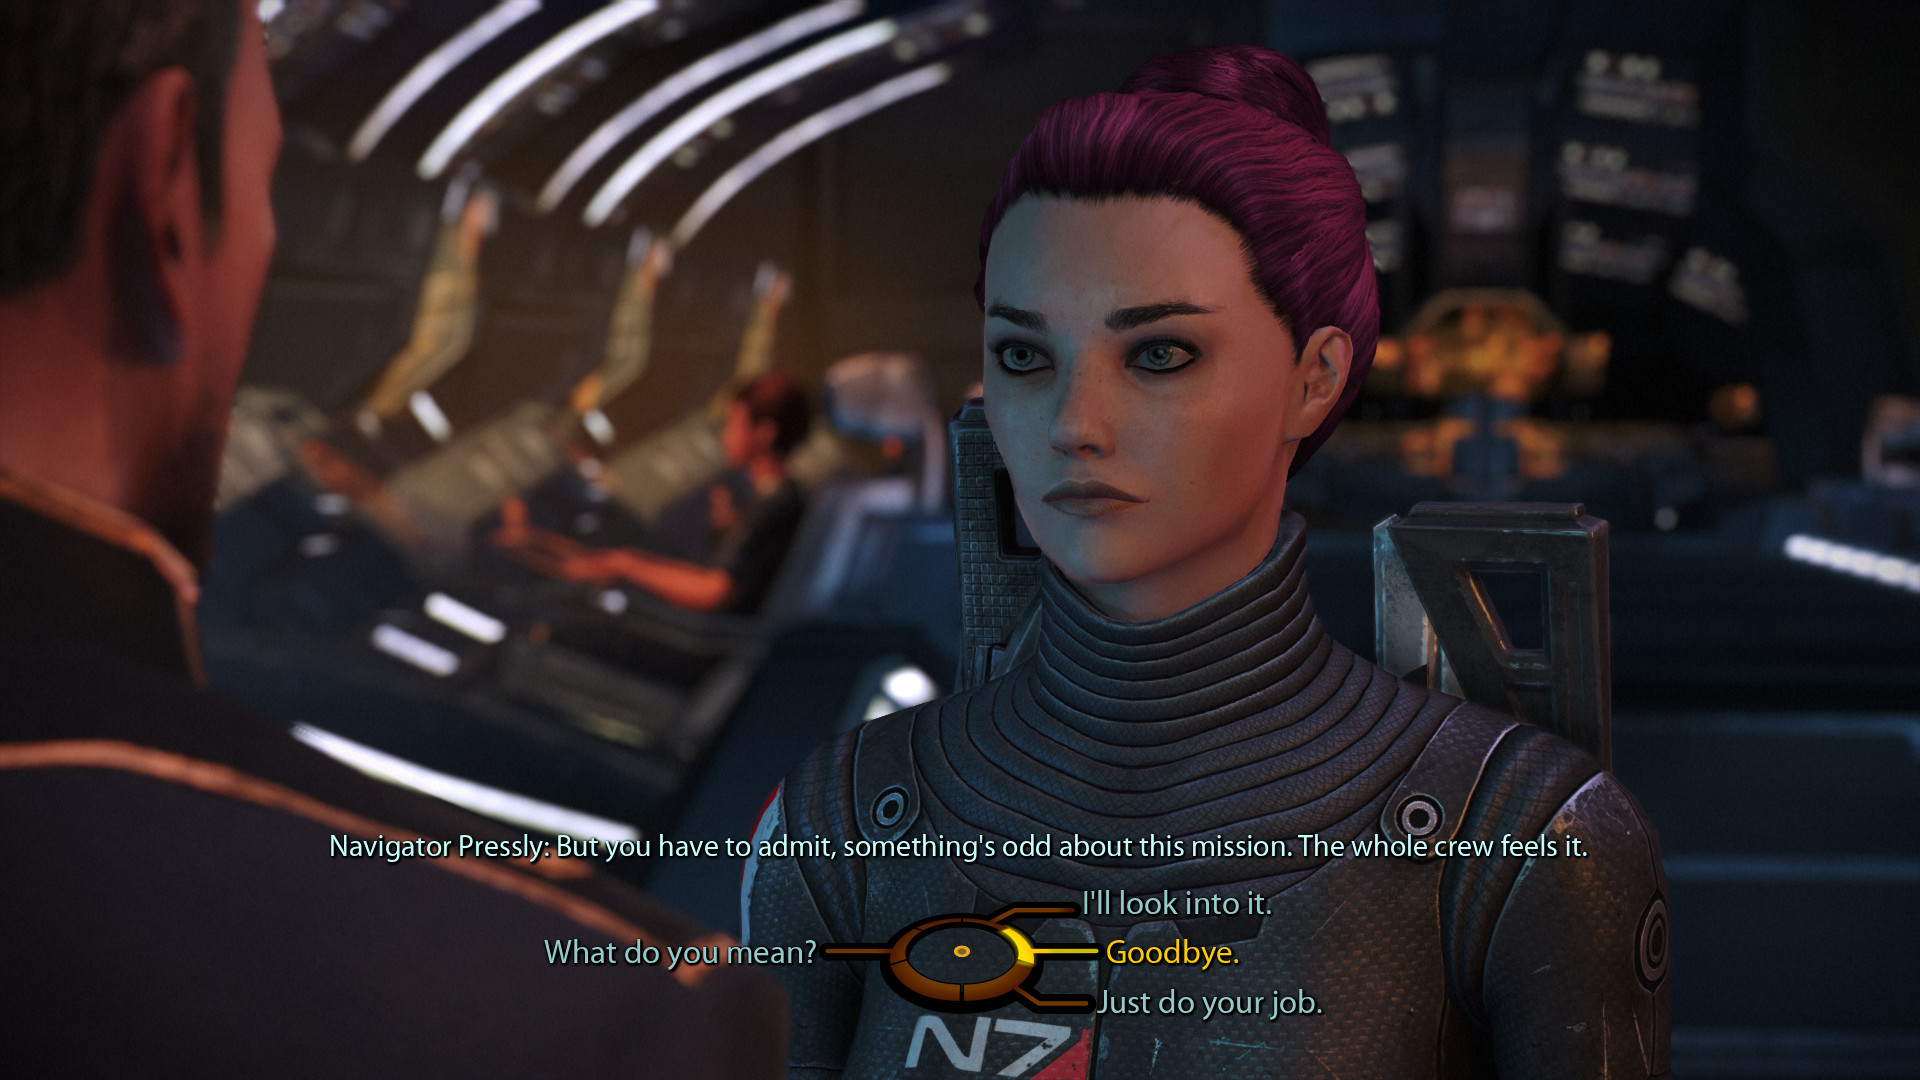
\includegraphics[width=1\textwidth]{images/me}
\caption{Przykład koła dialogowego w grze Mass Effect}
\label{fig:wheel}
\end{figure}

\begin{figure}[h]
\centering
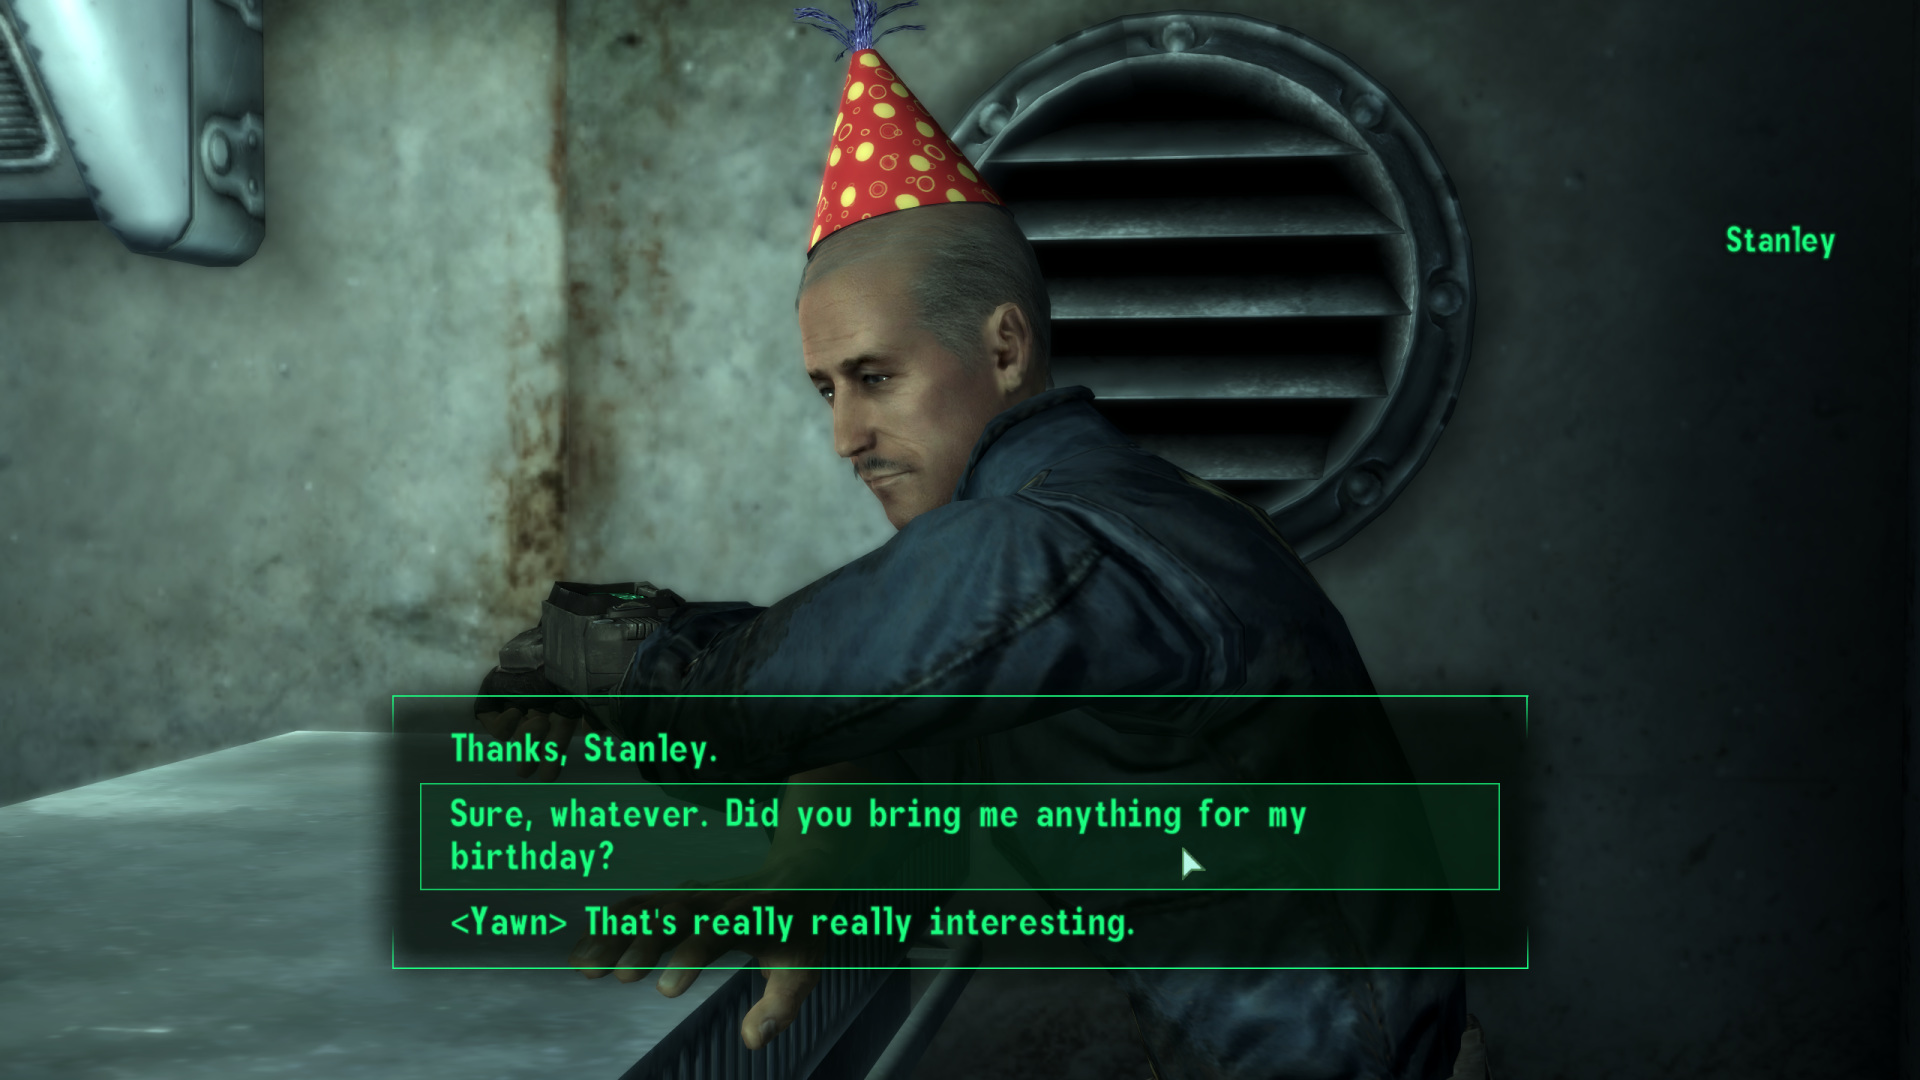
\includegraphics[width=1\textwidth]{images/fallout3}
\caption{Kadr z gry Fallout 3 przedstawiający przykładowy dialog}
\label{fig:fallout}
\end{figure}


\section{Model sztucznej inteligencji przeciwników w grach RTS (Bartosz Strzelecki)}
W sferze gier RTS sztuczna inteligencja (ang. artificial intelligence, AI) odgrywa kluczową rolę, wspierając doświadczenia z rozgrywki.
W tym przypadku termin odnosi się do zbioru algorytmów i systemów zaprojektowanych w celu symulacji
zachowań podobnych do tych gracza. Między innymi umiejętność podejmowania decyzji i rozwiązywania problemów.

Sztuczna inteligencja przeciwników w grach takich jak Warcraft III lub StarCraft II, przede wszystkim w trybie kampanii,
jest odpowiedzialna za kontrolowanie wrogich jednostek w celu zaoferowania graczowi wyzwania. Głównym zadaniem AI jest zasymulowanie
strategicznych decyzji i wydajne zarządzanie zasobami.
AI podejmuje decyzję na podstawie predefiniowanych zasad i algorytmów. Analizuje sytuację, w której się znajduje, biorąc pod uwagę
siłę swojej własnej armii, siłę armii gracza oraz specjalne zdolności jednostek i środowisko, w którym toczy się gra.
Ta analiza pozwala komputerowi na podejmowanie strategicznych decyzji jak na przykład, kiedy atakować, bronić się, eksplorować oraz rozszerzać swoje terytorium.
W tych grach sztuczna inteligencja może przybrać jeden z kilku wariantów wynikających z poziomu trudności. Wyższe poziomy
dają przeciwnikowi przewagę taką, jak wydajniejsze zbieranie zasobów lub szybsza produkcja jednostek.

W grze Warcraft III w trybie kampanii zachowanie przeciwników jest zaprojektowane z myślą o zanurzeniu gracza w fabularnej opowieści, jednocześnie
prezentując wciągające wyzwania związane z rozgrywką. Akcje wykonywane przez sztuczną inteligencję są dostosowane do celów danej misji, co pozwala
na dopasowanie do obowiązującej narracji.
Początkowo przeciwnik konstruuje i rozbudowuje swoją bazę, w celu zgromadzenia odpowiedniej liczby zasobów, szkolenia jednostek i prowadzenia badań.
AI strategicznie rozmieszcza budynki i struktury obronne, aby ochronić swoją fortecę przed najazdami gracza. 
Misje kampanii często też zawierają oskryptowane wydarzenia lub walki, które dodają głębi rozgrywce. Podczas tych starć wroga sztuczna inteligencja
może zachowywać się w specjalny sposób, kontrolując potężne jednostki, do których gracz normalnie nie ma dostępu lub inicjując działania, które popychają
narrację do przodu. Te wyreżyserowane wydarzenia tworzą niezapomniane chwile i jeszcze bardziej wciągają gracza w fabułę kampanii.
Zachowanie wroga w kampanii jest zróżnicowane i obejmuje różnorodne cele misji i scenariusze. Gracze mogą napotkać wrogów, którzy preferują agresywne ataki,
inni skupiają się na strategiach obronnych lub specjalizują się w taktyce hit and run. Sztuczna inteligencja dostosowuje proces podejmowania decyzji do
konkretnych wymagań misji, często wykorzystując ukształtowanie terenu, synergię jednostek i scenariusze wydarzeń, aby rzucić wyzwanie umiejętnościom gracza.
Ogólnie rzecz biorąc, zachowanie wrogów w kampanii Warcraft III ma na celu zapewnienie dynamicznego i wciągającego doświadczenia. Gracze muszą 
wykorzystywać myślenie strategiczne, zarządzanie zasobami i efektywny skład jednostek, aby przezwyciężyć różnorodne strategie stosowane przez wrogą sztuczną inteligencję.

\section{Mechanizm budowania oraz zarządzanie zasobami w grach RTS (Bogna Lew)}\label{s:budowanie}
Jednym z typowych elementów gier strategii czasu rzeczywistego  jest tworzenie baz i budowanie fortyfikacji. Mechanizm
ten stanowi urozmaicenie rozgrywki i wprowadza dodatkowe aspekty możliwe do uwzględnienia w planowaniu strategii. Dla
wielu gier RTS jest wręcz nieodłącznym elementem, który umożliwia graczowi tworzenie i rozwój nowych jednostek,
produkcję zasobów, umacnianie swojej pozycji oraz zwiększanie swojej potęgi.

Mechanizm ten wiąże się z szeregiem ograniczeń, które mają kluczowy wpływ na rozgrywkę. Należą do nich między innymi
ograniczenia związane z ukształtowaniem terenu oraz obecnością innych elementów scenerii. Każde z tych ograniczeń ma
swoje źródło w prawdziwym świecie i mechanizm budowania musi je uwzględniać.

Z tą mechaniką związany jest system zasobów, który jest popularnym aspektem gier z tego gatunku. Wiele gier strategii
czasu rzeczywistego umożliwia graczowi budowanie własnej ekonomii. Uzyskane przez niego zasoby często mogą zostać
wykorzystane przez mechanizm budowania jako koszta budowy obiektów.

Przykładem gry strategii czasu rzeczywistego implementującej tę mechanikę jest \textit{Warhammer 40,000: Dawn of War}\footnote{\url{https://www.dawnofwar.com/}}. Jest to
gra, której realia są osadzone w uniwersum gry bitewnej \textit{Warhammer 40,000}. Udostępnia ona tryb jednoosobowy oraz
wieloosobowy dla maksymalnie sześciu graczy. W pierwszym wariancie gracz wciela się w postać dowódcy
armii Space Marines z Blood Ravens i ma za zadanie zapobiec inwazji Orków. Gra \textit{Warhammer 40,000: Dawn of War} bardzo szybko
zyskała na popularności i oferowała wszystko, co było potrzebne dla tego gatunku. Z tego powodu warto się jej przyjrzeć,
pomimo faktu, że jej realia znacząco odbiegających od tych, w których zostanie osadzona tworzona przez nas gra.

\textit{Warhammer 40,000: Dawn of War} wyróżnia model pozyskiwania surowców. W grze dostępne są dwa rodzaje: Energia, która jest
generowana przez dedykowane do tego budowle oraz Rekwizycja, której szybkość wytwarzania jest uzależniona od kontrolowanych
przez gracza punktów strategicznych. Taka mechanika znacznie lepiej wpasowuje się w realia gry oraz wymusza na użytkowniku
przyjęcie agresywniejszej strategii.

Dodatkowo \textit{Warhammer 40,000: Dawn of War} posiada typowy dla gier RTS mechanizm tworzenia budowli. Gracz ma
do dyspozycji jednostki, którym może zlecić budowę wybranego przez siebie obiektu po poniesieniu kosztów jego utworzenia.
Zanim będzie możliwe rozpoczęcie budowania użytkownik musi wybrać miejsce, w którym budynek powstanie, co robi, przesuwając
jego podgląd po mapie. W tym czasie gra dokonuje walidacji miejsca i informuje gracza czy wybrany obszar jest poprawny,
odpowiednio podświetlając widok budynku. Wybudowanie obiektu nie jest natychmiastowe, co sprawia, że gra lepiej oddaje
realia, w których jest osadzona.

\begin{figure}[h!]
    \centering
    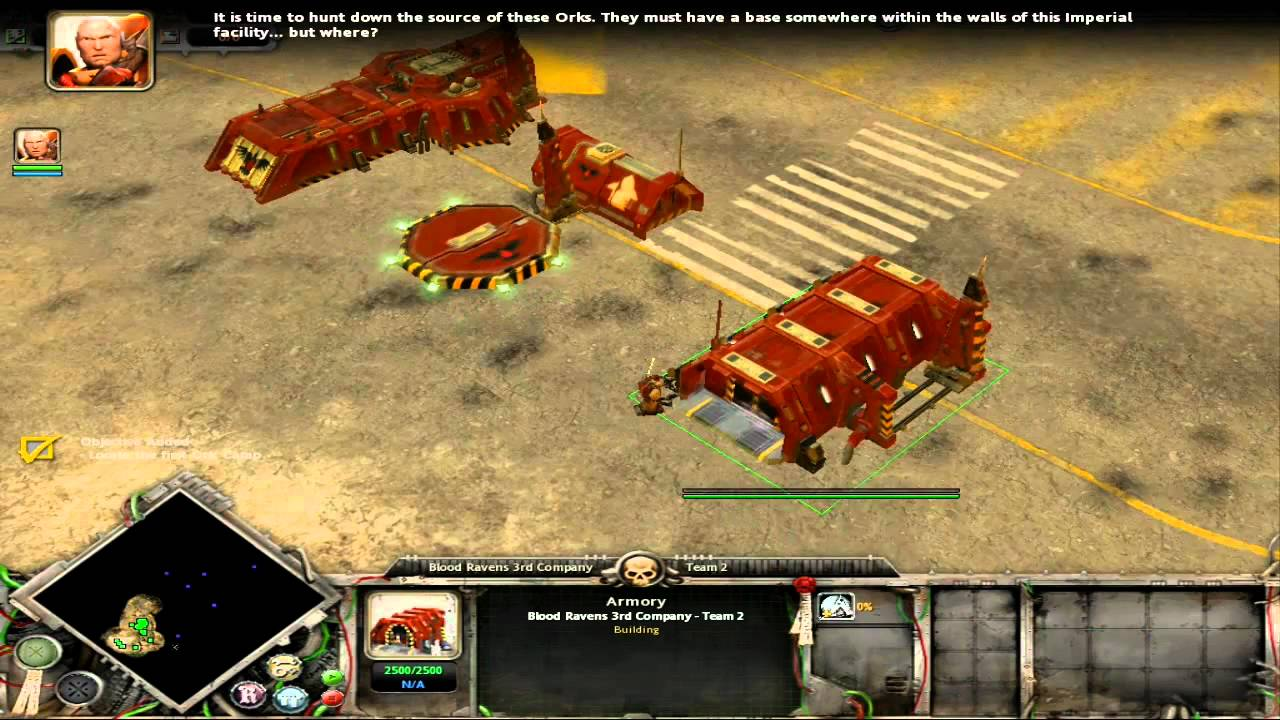
\includegraphics[width=1.0\textwidth]{images/warhammer1.jpg}
    \caption[Budowanie budynku przez dedykowaną do tego jednostkę w grze \textit{Warhammer 40,000: Dawn of War}.]{Budowanie budynku przez dedykowaną do tego jednostkę w grze \textit{Warhammer 40,000: Dawn of War}\protect\footnotemark.}
\end{figure}
\FloatBarrier
\footnotetext{Internet, \url{https://www.youtube.com/watch?v=wNtnGFoVReU}, dostęp: 19.11.2023}

\section{Mechanizm walki oraz zarządzania ekwipunkiem w Kingdom Come: Deliverance [Bogna Lew]}

Kingdom Come: Deliverance to gra z gatunku RPG osadzoną w realiach Europy Środkowej na początku XV wieku. Chociaż nie
jest to gra czasu rzeczywistego to jest to pozycja warta wymienienia ze względu na dbałość twórców o zachowanie realizmu
epoki oraz staranność wykonania mechanizmów walki oraz zarządzania ekwipunkiem. Jest ona przeznaczona dla jednego gracza,
a całość zaprezentowana jest z perspektywy pierwszoosobowej. W trakcie rozgrywki użytkownik rozwija swoją postać, bierze
udział w starciach, prowadzi rozmowy z niezależnymi postaciami i wiele więcej.

Godny uwagi jest mechanizm walki. Twórcy skupili się na jak najdokładniejszym oddaniu średniowiecznego stylu walki. W tym
celu skrupulatnie przestudiowali w jaki sposób władano mieczem w tamtych czasach, a następnie w pełni oddali to w grze.
Wykorzystali do tego tysiące animacji oraz starannie oddali fizykę pojedynków. W efekcie powstał realistyczny mechanizm
walki, który umożliwia graczowi parowanie, zadawanie ciosów oraz blokowanie.

Kolejnym elementem wartym wymienienia jest rozbudowany system zarządzania ekwipunkiem. Przeznaczony do tego panel jest
podzielony na dwie sekcje - jedna w której wyświetlona jest lista posiadanych rzeczy oraz druga przeznaczona na postać
gracza. Może on dowolnie spersonalizować swoją postać, poprzez możliwość założenia wielu elementów ubioru naraz tworząc
warstwy.  Dodatkowo, każdy przedmiot posiada swoją wagę, a postać swój maksymalny udźwig. W przypadku przekroczenia limitu
gracz zostaje ukarany poprzez spowolnienie ruchów w walce i uniemożliwieniu biegania. Jest to wzorowane na rzeczywistości,
dzięki czemu gra jeszcze lepiej oddaje realia epoki.

\section{Sterowanie jednostkami w grze Mount\&Blade (Zofia Sosińska)}\label{chap:mb}

Mount\&Blade jest to gra komputerowa z gatunku cRPG (komputerowa gra fabularna, ang. computer role-playing game) z elementami strategicznymi, stworzona przez turecką firmę TaleWorlds Entertainment i wydana przez Paradox Interactive. W otwartym świecie fikcyjnej krainy Calradia, stylizowanej na czasy średniowieczne, gracz ma pełną dowolność stylu rozgrywki. W jego mocy jest zarówno zbieranie armii i dążenie do zostania królem, jak i zostanie wasalem jednego z władców. Za pomocą dialogów i walk z postaciami gracz buduje unikatową historię.
Jedną z wartych uwagi mechanik, zaimplementowaną w grze Mount\&Blade, jest sterowanie jednostkami służącymi granemu charakterowi. Gracz bezpośrednio kieruje jedynie główną postacią. Podczas walki reszcie może wydawać rozkazy. Poprzez cyfry 0-4 wybiera grupę, do której się odnosi np. łuczników. Następnie przez klawisze F1-F11 wydaje konkretny rozkaz np. odwrót. Sztuczna inteligencja postaci zajmuje się już samym wykonaniem czynności. Gracz nie martwi się, czy jednostki znajdą optymalną drogę, będą celować w przeciwników, czy z nimi walczyć.


\section{Kompasy w grach (Zofia Sosińska)}\label{chap:skrm}
Częstą funkcjonalnością gier jest możliwość eksploracji świata, w którym na gracza czekają przygody i zadania do wykonania.
Jednak przestrzeń przygotowana dla użytkownika może być na tyle duża i skomplikowana, że powstaje ryzyko 
zgubienia się. Jednym ze sposobów jakim projektanci gier wyciągają rękę do zatraconego w labiryncie użytkownika jest danie mu
kompasu. Może to być bardzo proste narzędzie, pokazujące jedynie strony świata, immitujące klasyczny przedmiot ze świata rzeczywistego.
Już taka garstka informacji potrafi uprościć graczowi odnalezienie drogi do celu. Jednak innym podejściem jest rozrzerzenie 
funkcjonalności kompasu o pokazywanie pozycji innych ważnych punktów odniesienia, celów, do których trzeba się dostać, lub 
kluczowych posatci.

The Elder Scrolls V: Skyrim (skrótowo Skyrim) jest to fabularna gra
wyprodukowana przez Bethesda Game Studios i wydana przez Bethesda Softworks. Autorzy przygotowali dla gracza duży świat,
który ten może dowolnie eksplorować. Nawigację oparli o bardzo pomocne i sprytne rozwiązanie,
jakim jest pasek przedstawiający pole widzenia gracza. Służy on między innymi jako kompas, ponieważ 
jedną z jego mechanik jest pokazanie użytkownikowi stron świata, znajdujących się w kierunku, w którym 
on patrzy. Pasek ułatwia także poruszanie się po świecie, sygnalizując położenie wrogów, kompanów i ważnych 
dla rozgrywki lokalizacji.

\begin{figure}[htbp]
	\centering
	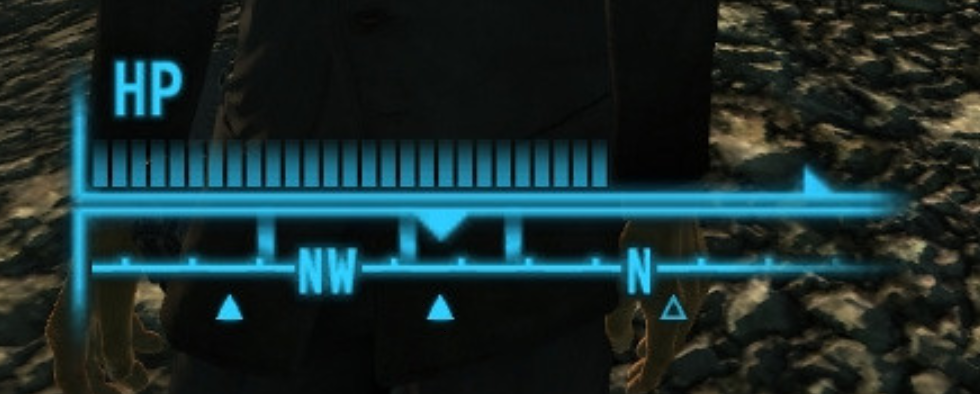
\includegraphics[width=0.9\textwidth]{images/ui/compassSkyrim.png}
	\caption{Kompas z gry Skyrim}\label{fig:Fallout}
\end{figure}


\section{Stawianie budowli (Zofia Sosińska)}\label{chap:omd}
Jedną z kluczowych mechanik gier z gatunku RTS jest budowanie budynków. Funkcjonalność pozwala graczowi 
na podejmowanie strategicznych decyzji w zależności od potrzeb i możliwości budowli. Funkcje pełnione 
przez budynek mogą być bardzo różnorodne. W niektórych przypadkach ich zadaniem jest produkcja surowców, czy leczenie
jednostek, ale są i takie, które skupiają się na wspieraniu w obliczu bitwy. Mogą to być fortyfikacje opóźniające natarcie,
bądź chociażby machiny wojenne towarzyszące ofensywie.

Orcs must die! to strategiczna gra akcji stworzona i wydana przez studio Robot Entertainment. Zadaniem gracza jest wcielenie się
w jednego z  Wojennych Magów i mordowanie nadciągających grup orków za pomocą różnorodnych broni i mechanizmów, które może postawić.
W przejrzysty sposób zostało rozwiązane samo wyświetlenie dostępnych do zbudowania pułapek. Na dole ekranu pokazują się wizerunki mechanizmów,
które może postawić oraz informacja o ich cenie. Naciskając odpowiedni numer na klawiaturze, gracz wybiera, co chce zbudować. Po zatwierdzeniu lewym przyciskiem myszki,
budynek pojawia się w zaznaczonym miejscu. Od tego momentu pułapka będzie pomocą dla głównej postaci podczas zwarcia z przeciwnikami.
Jego ograniczeniem w stawianu mechanizmów są jego fundusze, dlatego musi przemysleć, co kupić oraz gdzie najoptymalniej będzie to postaawić.

\begin{figure}[h!tbp]
    \centering
    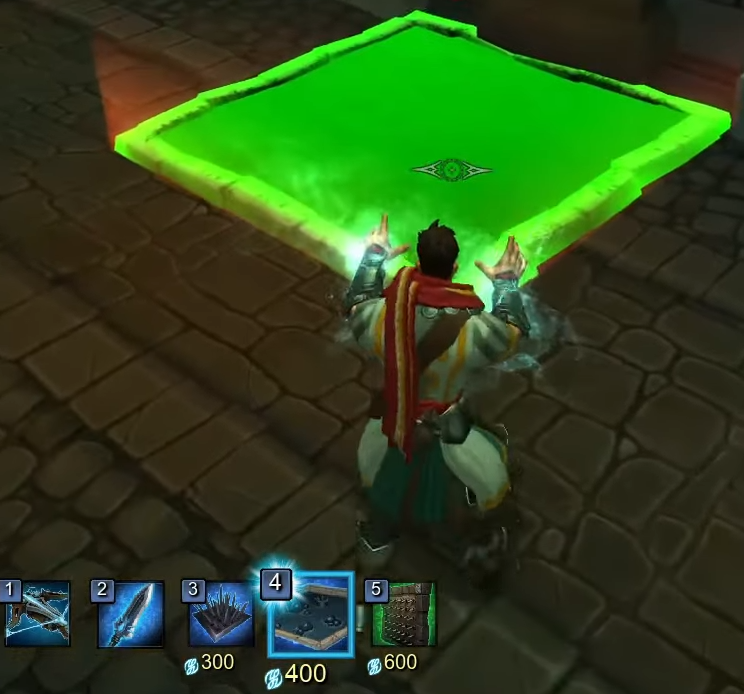
\includegraphics[width=0.9\textwidth]{images/ui/buoildingsOrcs.png}
    \caption{Wyświetlenie dostępnych pułapek w Orcs must die!}\label{fig:Orcs}
\end{figure}
\chapter{Wprowadzenie do dziedziny}\label{chap:field}




\section{Podrozdział}
Lorem ipsum dolor sit amet, consectetur adipiscing elit. In semper, sem id aliquam consectetur, nulla enim ornare erat, vitae lacinia odio enim sagittis leo. Nunc vestibulum lorem sem, a pharetra orci volutpat a. Nullam quis fermentum dolor. Sed quam nisl, imperdiet quis leo quis, sollicitudin dictum nisi. Vivamus orci mauris, convallis eget blandit eget, convallis sed est. Nullam a ex in ex ultricies suscipit nec a purus. Morbi tincidunt libero et magna mollis, in posuere quam maximus. Donec commodo nunc orci, ut convallis nulla congue ac. Pellentesque pulvinar semper aliquet. Mauris ac libero vel ante ullamcorper vulputate sed id diam. Vivamus lobortis orci non nunc lobortis, ac varius est scelerisque. Integer ut nibh est. Phasellus nec dui luctus, porttitor nulla ac, commodo lectus. Vestibulum vehicula aliquam sem, quis accumsan nibh vulputate sed. Obrazek kawusi to rys.\ref{fig:coffee}~\cite{dx12_2}.

\begin{figure}[htbp]
    \centering
    
\includegraphics[width=0.9\textwidth]{images/kawunia.png}
    \caption{Smacznej kawuni}\label{fig:coffee}
\end{figure}

Nunc venenatis in felis lobortis vehicula. Praesent consequat aliquam mollis. Cras sed interdum lectus, eget maximus ipsum. Praesent sollicitudin nisi eros, et pellentesque nisi fermentum non. Orci varius natoque penatibus et magnis dis parturient montes, nascetur ridiculus mus. Maecenas in volutpat sapien, eget mattis orci. Nulla tellus ligula, blandit nec lorem nec, eleifend condimentum ante.

Cras ultricies leo ipsum, ut sodales augue mattis ut. Nam aliquam blandit felis, posuere blandit felis rutrum in. Aenean feugiat sodales leo ut pulvinar. Maecenas vel scelerisque ex, vitae feugiat ante. Donec porta tincidunt dapibus. Sed sed pharetra tellus, a gravida quam. Donec euismod risus vitae turpis commodo, porta eleifend diam porta. Nullam sagittis gravida dolor, in blandit velit ornare in. Proin quis accumsan mi, sed consequat purus. Integer vitae imperdiet diam. Donec nec congue urna, sit amet tempus justo. Etiam pharetra pellentesque libero in tincidunt. Integer tristique tempor enim et malesuada. Donec accumsan lacus ut ligula mollis imperdiet. Maecenas malesuada dui eu egestas fermentum. Fusce rhoncus faucibus elit sit amet fermentum.

Nunc vehicula vel mi vel rhoncus. Curabitur euismod, arcu id faucibus rutrum, arcu leo consectetur sapien, ac ultricies mi erat sed velit. Nunc vitae quam eget eros facilisis hendrerit vitae non nibh. Duis dui orci, bibendum cursus libero id, tempor consectetur purus. Vivamus sit amet viverra lorem. Vivamus id tincidunt lectus. Sed varius feugiat enim, non aliquet urna fermentum eu. Integer vestibulum velit sit amet metus consectetur dapibus. Vestibulum sagittis eu magna a porttitor. Cras dapibus ipsum at urna condimentum, quis ornare sem vulputate. Suspendisse efficitur sit amet odio nec rhoncus. Donec venenatis urna velit, et aliquam neque molestie sit amet. Nulla vulputate accumsan metus. Donec vel tortor mauris. Fusce sit amet leo ut tortor commodo accumsan at et turpis. Ut hendrerit elit in nisl posuere viverra.

In hac habitasse platea dictumst. Curabitur id nibh ut nisl vehicula interdum. Fusce diam eros, scelerisque at fermentum nec, eleifend non erat. In pharetra mauris purus, ac malesuada neque suscipit id. Vestibulum placerat orci in dui lacinia, in porta urna consectetur. Etiam feugiat vehicula nulla, eget scelerisque velit malesuada in. Donec nec rhoncus ex. Orci varius natoque penatibus et magnis dis parturient montes, nascetur ridiculus mus. Donec tincidunt ex sed urna maximus, vel dapibus arcu venenatis. Cras posuere nisl erat. Vestibulum ante ipsum primis in faucibus orci luctus et ultrices posuere cubilia curae; Sed posuere neque et pretium congue. Cras at nisl sit amet dui varius feugiat. Nulla nec leo ut lacus pharetra placerat quis quis velit. Ut id hendrerit magna, ut sollicitudin diam.

Aenean varius bibendum odio, eu dapibus ipsum vulputate iaculis. Aliquam nec eleifend dui. Nunc vel eros vitae risus tincidunt fermentum in at ex. Etiam leo leo, ultricies et ultricies nec, tristique accumsan odio. Quisque nibh quam, sollicitudin quis aliquam eget, laoreet sit amet enim. Pellentesque eget sollicitudin justo, sed lobortis nisl. Orci varius natoque penatibus et magnis dis parturient montes, nascetur ridiculus mus. Cras consectetur turpis ut ipsum elementum, vel feugiat dui dapibus. Maecenas est metus, accumsan vel dolor rutrum, rutrum porttitor lectus. Curabitur nec finibus sapien. Nam non rutrum magna, at tempor massa. Morbi nec congue sem. Curabitur rutrum dolor eu diam mattis, ut ultrices ipsum auctor.

\chapter{Technologie, algorytmy i narzędzia}
\section{Przegląd silników gier (Bogna Lew)}\label{s:silniki}
Silnik gier komputerowych jest oprogramowaniem służącym głównie do wytwarzania gier komputerowych. Dostarcza podstawowe
narzędzia, takie jak biblioteki czy edytor poziomów, dzięki którym łatwiej można dokonywać zmian w grze. Wybranie
odpowiedniego silnika przed rozpoczęciem pracy ma kluczowy wpływ na proces wytwórczy i efekt końcowy.

Obecnie dostępnych jest wiele silników, a każdy z nich ma różne możliwości. W celu uproszczenia wyboru zdecydowaliśmy
się zawęzić listę do trzech najpopularniejszych obecnie darmowych silników, czyli Godot, Unity oraz Unreal Engine.

Pierwszy z nich jest w pełni darmowym silnikiem open source. Posiada prosty i intuicyjny interfejs, a w Internecie
tworzone jest przez społeczność wiele samouczków. Nie posiada on jednak oficjalnej dokumentacji oraz jest zdecydowanie
mniej popularny od pozostałych dwóch.

Kolejny silnik, Unity jest określany jako przyjazny dla początkujących. Posiada bogatą dokumentację oraz jest dostępnych
dużo samouczków stworzonych przez jego społeczność. Unity świetnie się nadaje do tworzenia gier 3D. Silnik ten jest
dostępny w wersji bezpłatnej oraz oferującej więcej możliwości wersji płatnej. Co więcej, ma możliwość rozszerzenia
o dodatkowe narzędzia dostępne w Asset Store.

Ostatni z silników jest najbardziej kojarzony z grami AAA. Cechuje go zaawansowana grafika, która umożliwia wytwarzanie
fotorealistycznych gier. Korzystanie z niego jest darmowe, a opłata w wysokości 5\% jest naliczana jedynie, gdy gra
zarobi ponad milion USD.

Tabela \ref{fig:teng} przedstawia porównanie wymienionych silników w istotnych, z punktu widzenia projektu, aspektach.

\begin{table}[h]
\caption{Porównanie silników.}
\begin{center}
\begin{tabular}{ |c||c|c|c| }
 \hline
 Silnik & Unity & Unreal Engine & Godot \\
 \hline \hline
 Popularność & duża & duża & mała \\
 \hline
 3D & Tak & Tak & Tak \\
 \hline
 Język & C\# & C++ & C\#, C++, GDScript \\
 \hline
 Baza wiedzy & dokumentacja, samouczki & dokumentacja, samouczki & samouczki, fora \\
 \hline
 Open source & Nie & Nie & Tak \\
 \hline
\end{tabular}
\end{center}
\label{fig:teng} 
\end{table}

Finalnie zdecydowaliśmy się na implementację gry w Unity, ponieważ jest to silnik, który najlepiej odpowiada wymaganiom projektu.

\chapter{Projekt systemu}
\section{Modelowanie terenu (Bogna Lew)}
Do utworzenia terenu do gry wykorzystaliśmy zasób 3D World Building udostępniany przez Unity. Umożliwia on automatyczne generowanie terenu na podstawie heightmapy - monochromatycznego obrazu reprezentującego model wysokościowy. Kolor czarny reprezentuje najniższe punkty, natomiast kolor biały -  najwyższe.

\begin{figure}[h!]
    \centering
    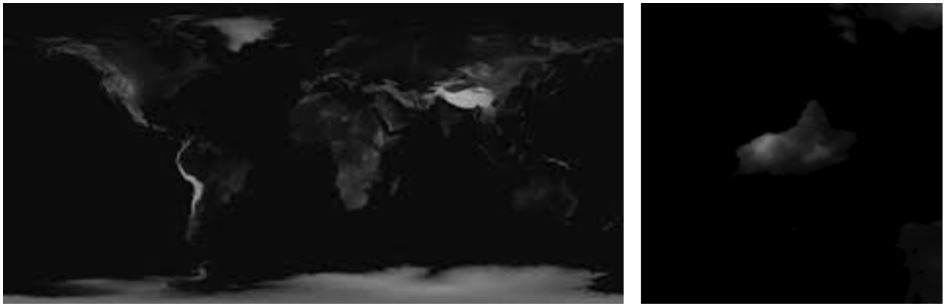
\includegraphics[width=0.9\textwidth]{images/modelowanie_terenu/przykladowe_heightmapy.jpg}
    \caption{Przykładowe heightmapy}\label{fig:przykladowe_heightmapy}
\end{figure}

Wygenerowanie terenu umożliwia narzędzie Terrain Toolbox, które można uruchomić wybierając z menu Window -> Terrain -> Terrain Toolbox. Pozwala ono na ustawienie podstawowych parametrów takich jak długość, szerokość oraz wysokość terenu. Należy również zaznaczyć checkbox Import Heightmap oraz załączyć obraz z modelem wysokościowym. Na koniec trzeba nacisnąć przycisk Create, co spowoduje dodanie do sceny wygenerowanego terenu.

\begin{figure}[h!]
    \centering
    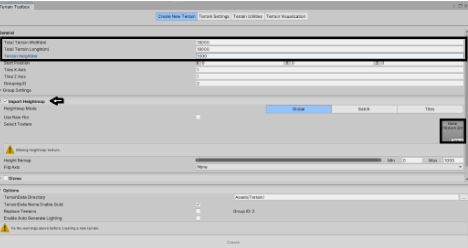
\includegraphics[width=0.6\textwidth]{images/modelowanie_terenu/generowanie.jpg}
    \caption{Widok na panel narzędzia Terrain Toolbox z zaznaczonymi wymienionymi sekcjami.}\label{fig:generowanie_terenu}
\end{figure}

Tak utworzony teren, chociaż już jest grywalny, posiada ostre i postrzępione krawędzie, które nie wyglądają zbyt estetycznie. Wygładzenie ich poprawi wygląd terenu i sprawi, że będzie on bardziej realistyczny. Do tego służy narzędzie Smooth Height dostępne w inspektorze terenu. Powoduje ono uśrednienie pobliskich płaszczyzn, co pozwala na usunięcie nagłych zmian terenu i w rezultacie wygładzenie go.

\begin{figure}[h!]
    \centering
    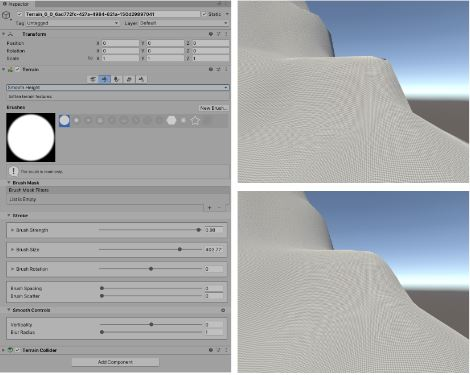
\includegraphics[width=0.8\textwidth]{images/modelowanie_terenu/rzezbienie.jpg}
    \caption{Widok panelu inspektora oraz terenu przed (górny) i po (dolny) zastosowaniu narzędzia Smooth Terrain.}\label{fig:rzezbienie_terenu}
\end{figure}

Kolejnym krokiem jest nałożenie tekstur. Służy do tego narzędzie Paint Texture. Umożliwia ono dodanie warstw, którymi będzie można pokolorować teren. Warstwa znajdująca się najwyżej jest uznawana za domyślną i jej tekstura zostanie nałożona na cały teren. Pozostałe warstwy natomiast stanowią swego rodzaju paletę kolorów, którymi można pomalować teren za pomocą pędzla, który można wybrać w zakładce Brushes. W zakładce Stroke można ustawić podstawowe parametry pędzla takie jak Brush Size oraz Brush Strength. Pierwszy parametr odnosi się do rozmiaru pędzla, a co za tym idzie obszaru na który dana tekstura zostanie nałożona, natomiast drugi pozwala na określenie w jakim stopniu nakładany materiał zakryje już nałożony.

\begin{figure}[h!]
    \centering
    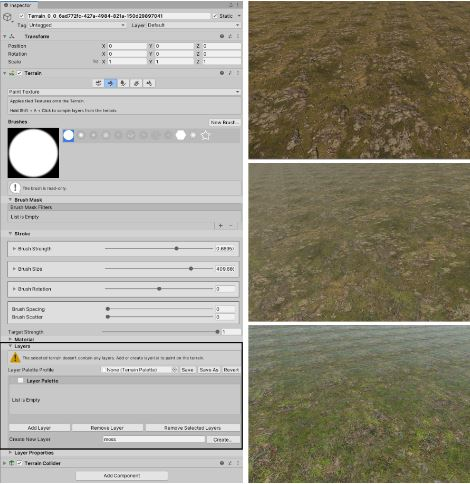
\includegraphics[width=0.8\textwidth]{images/modelowanie_terenu/tekstury.jpg}
    \caption{Widok panelu inspektora z wybranym narzędziem Paint Texture oraz efektu przed nałożeniem 2 tekstury (górny zrzut), po nałożeniu tekstury gdy Brush Strength wynosi 0.26 (środkowe zdjęcie) oraz gdy wynosi 0.67 (dolne).}\label{fig:malowanie_tekstur}
\end{figure}

Kolejną opcją udostępnianą przez Unity jest możliwość automatycznego ustawienia obiektów na mapie w losowy sposób, dzięki narzędziu Paint Trees. Do udostępnianych przez nie parametrów należą między innymi Brush Size, działający analogicznie jak poprzednio, oraz Tree Density, które definiuje średnią liczbę drzew umieszczanych na zdefiniowany obszar. Obok przedstawiono przykładowy rezultat. Wykorzystano do tego paczkę LowPoly Trees and Rocks dostępną w Unity Assets Store.

\begin{figure}[h!]
    \centering
    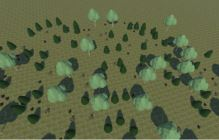
\includegraphics[width=0.5\textwidth]{images/modelowanie_terenu/drzewa.jpg}
    \caption{Widok na teren z drzewami.}\label{fig:pomalowane_drzewa}
\end{figure}

\begin{figure}[h!]
    \centering
    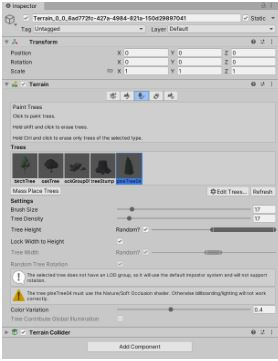
\includegraphics[width=0.6\textwidth]{images/modelowanie_terenu/malowanie_drzew.jpg}
    \caption{Widok na inspektor z włączonym narzędziem Paint Trees.}\label{fig:malowanie_drzew}
\end{figure}



Do stworzenia interfejsu użytkownika (UI) za wzorce użyliśmy gier “Mount&Blade”, “Mount&Blade2 Bannerlord”, “Warcraft3”, “The Elder Scrolls V: Skyrim”, “Orcs must die”aby umożliwić graczowi jak najprzyjemniejszą rozrywkę oraz wszystkie potrzebne funkcje.

Pierwszy ekran
Wzorowanie: “Mount&Blade”
Jako pierwszy ekran, który widzi gracz przewidujemy grafikę z możliwością wybrania jednej z opcji z menu głównego.

Poruszanie się

Przewidujemy:
górny pasek z najważniejszymi informacjami:surowce, fundusze, czas, kompas
ikony postaci, na które gracz może się przełączyć;
obszar dla komentarzy
pasek życia.

Inspiracja dla górnego paska z najważniejszymi informacjami:surowce, fundusze, czas oraz ikon postaci, na które gracz może się przełączyć:

źródło: Warcraft 3

Inspiracja dla kompasu:

źródło: The Elder Scrolls V: Skyrim
Inspiracja dla obszaru dla komentarzy oraz pasek życia:

źródło: Mount&Blade2 Bannerlord

Rozmowa 

źródło: Mount&Blade

Walka
Przy walce dostępne materiały zamienią się na pasek pokazujący sumaryczne życie naszej drużyny i drużyny przeciwnej oraz możliwe komendy do wydania.


Inspiracja dla możliwych komend:
źródło: Mount&Blade

Budowa budynków
W tym trybie pokażą nam się dostępne do zbudowania budynki, a po wybraniu pojawią się przed nami. Po zatwierdzeniu budynek zostanie wybudowany.


Inspiracja dla trybu budowania:

źródło: Orcs must die

\section{Mechanizm budowania (Bogna Lew)}\label{s:bud_impl}

Opracowany mechanizm umożliwia graczowi na przełączenie się w tryb budowania poprzez naciśnięcie klawisza \texttt{B}, który od razu
wyświetli podgląd bazowego obiektu. Widok budynku przemieszcza się przed postacią oraz odpowiednio obraca się razem z
nią. Efekt poruszania się podglądu został uzyskany za pomocą poniższego wzoru:
\begin{equation}
\begin{cases}
x = r \times sin(\alpha) \\
y = 0 \\
z = r \times cos(\alpha)
\end{cases}
\end{equation}

gdzie $x$, $y$ i $z$ to współrzędne odpowiednio względem osi X, Y i Z, $r$ to odległość środka obiektu od postaci
gracza, natomiast $\alpha$ to kąt o jaki jest on obrócony względem osi Y.

Podgląd budynku będzie widoczny do czasu, aż gracz go umieści naciskając prawy przycisk myszy bądź wychodząc z trybu
edycji naciskając klawisz \texttt{Escape}. Jeżeli widok budowli znajduje się w poprawnym do umieszczenia miejscu to jest on
podświetlany na zielono, w przeciwnym razie - na czerwono. Wybudowanie powoduje przywrócenie bazowych kolorów obiektu
oraz włącza wykrywanie kolizji z nim, dzięki czemu budynek poprawnie oddziałuje z otaczającym go środowiskiem.

\begin{figure}[h!]
    \centering
    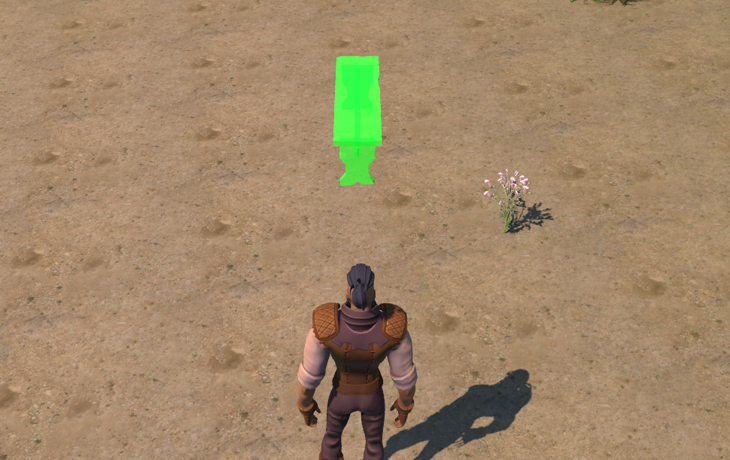
\includegraphics[width=1\textwidth]{images/implementacja/mechanizm_budowania/poprawne.png}
    \caption{Przykład podglądu w poprawnym umiejscowieniu.}
\end{figure}
\FloatBarrier

Do weryfikacji poprawności umiejscowienia budynku wykorzystano mechanizmy wyzwalacza (ang. \textit{trigger}) oraz rzucania
promienia (ang. \textit{raycasting}). Pierwszy z nich polega na wykrywaniu czy obiekt znalazł się w obszarze kolizji bez
brutalnego zatrzymywania go. Oznacza to, że może on przeniknąć przez inny element bez widocznych konsekwencji, jedynie
wysyłając sygnał, że dana sytuacja nastąpiła. Druga metoda natomiast polega na wypuszczeniu promienia o pewnej długości
w zadanym kierunku i sprawdzeniu, czy z czymś się zderzył.

Wyzwalacz został zastosowany do wykrywania kolizji z innymi obiektami na mapie, takimi jak postacie, czy elementy
scenerii niebędące terenem. W tym celu wykorzystano metody \verb|OnTriggerEnter()| i \verb|OnTriggerExit()|, które są wywoływane
odpowiednio gdy, dany obiekt znalazł się w obszarze kolizji innego elementu, bądź go opuścił. Każda z nich odpowiednio
zmienia poprzez zwiększenie bądź zmniejszenie wartości licznika kolizji obiektu. Jeżeli jego wartość jest różna od zera, tzn.
obiekt z czymś koliduje, to umiejscowienie jest uznawane za niepoprawne.

Drugi z mechanizmów został wykorzystany do sprawdzenia nachylenia podłoża. Efekt został osiągnięty poprzez rzucenie
promienia o niewielkiej długości z każdego z dolnych narożników obiektu i zliczeniu ile z nich wykryło kolizję z ziemią.
Brak wykrycia kolizji można zinterpretować jako zapadanie się bądź zbyt mocne lewitowanie danego narożnika nad
powierzchnią ziemi. Z tego powodu przyjęto, że jeśli co najmniej trzy z nich zderzyły się z podłożem, to umiejscowienie
jest poprawne.

\begin{figure}[h!]
    \centering
    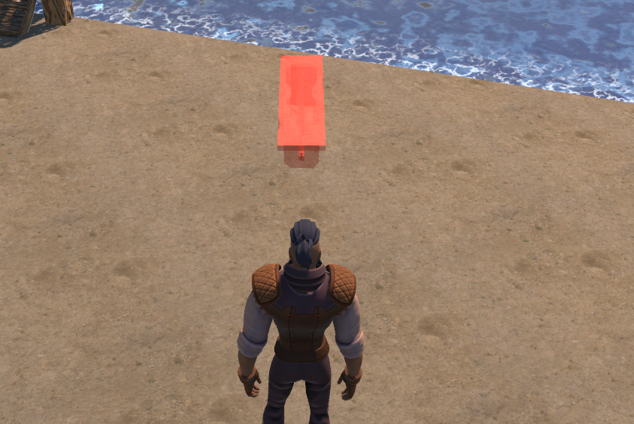
\includegraphics[width=1\textwidth]{images/implementacja/mechanizm_budowania/niepoprawne.png}
    \caption{Przykład podglądu w niepoprawnym umiejscowieniu.}
\end{figure}
\FloatBarrier

Dodatkowo metodę rzucania promienia wykorzystano do wykrycia kolizji z drzewami. Obiekty te są traktowane przez silnik
jako część terenu, przez co metoda wykorzystująca wyzwalacz pomija je. Dlatego w celu wykrywania kolizji z nimi
zdecydowano się na rzucenie dwóch grup promieni biegnących w głąb obiektu z naprzeciwległych krawędzi prostopadłych do
osi Y. Każdy z promieni biegnie w połowie wysokości obiektu i sięga przeciwnej ściany. Tak skomplikowany układ ma na
celu zapewnienie poprawności wykrywania kolizji w przypadku, gdy początki promieni znajdują się wewnątrz kolidującego
obiektu. Jeśli którykolwiek z nich zderzy się z drzewem, to wybrane miejsce jest uznawane za niepoprawne.

\begin{figure}[h!]
   \centering
   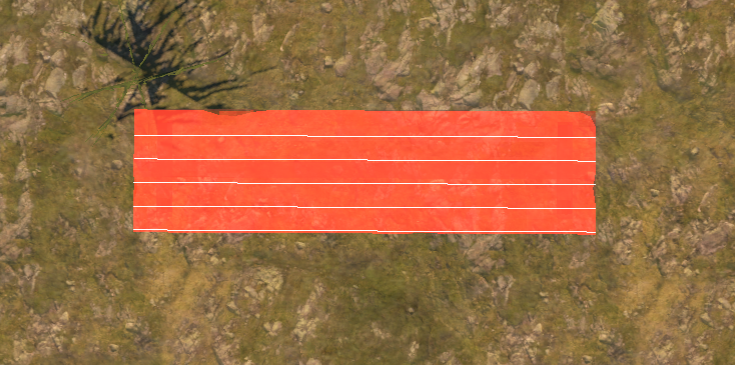
\includegraphics[width=1\textwidth]{images/implementacja/mechanizm_budowania/gizmos_drzewo_2.png}
   \caption{Widok z góry na siatkę promieni służących do wykrywania kolizji z drzewami.}
\end{figure}
\FloatBarrier
\begin{figure}[h!]
   \centering
   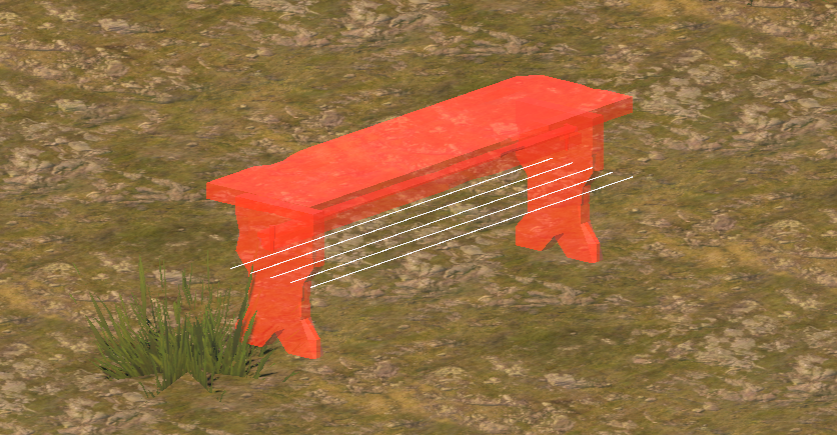
\includegraphics[width=1\textwidth]{images/implementacja/mechanizm_budowania/gizmos_drzewo_1.png}
   \caption{Widok z boku na siatkę promieni służących do wykrywania kolizji z drzewami.}
\end{figure}
\FloatBarrier

\section{Nawigacja (Zofia Sosińska)}\label{chap:naw}

Kluczowym dla gry założeniem jest ułatwienie graczowi wczucia się w realia świata, w którym się znajduje. 
Jako jeden z głównych warunków pogłębienia immersji uwypuklono brak implementacji mapy, na której gracz widziałby świat. 
W ten sposób nie upraszczamy mu poruszania się i odnajdywania lokacji tak,
jak i człowiek w realnym świecie w czasach średniowiecznych nie kierował się zapisanymi na kartce kartograficznymi obrazami, 
ale własną i zdobytą od innych wiedzą o otaczającym go terenie. 

Jedyną pomocą, jaką otrzyma gracz, będzie pasek obrazujący pole widzenia granej postaci.
Pierwszą rolą narzędzia będzie pokazanie kierunku świata, który znajduje się w polu widzenia gracza.
Zakładamy, że grana postać potrafi sama taką informację odczytać, chociażby z położenia Słońca.

Kolejną informacją na omawianym elemencie będzie miejsce, w którym znajduje się przeciwnik. 
Dotyczy to antagonistów widocznych w polu widzenia, jak i ukrytych za ścianą. 
Druga część będzie logicznie ponieważ zakładamy, że postać gracza może usłyszeć 
wroga za przeszkodą.


\section{Sterowanie jednostkami, podążanie za główną postacią (Zofia Sosińska)}\label{chap:sjpzgp}
Na samym początku gry stworzona przez gracza postać pojawia się sama. W tym momencie jest to jedyny obiekt, którym gracz może sterować.
Kontroluje, gdzie postać idzie, jak walczy oraz z kim rozmawia. Z biegiem czasu gra będzie jednak naciskać na formowanie drużyny,
ponieważ pokonywanie wielu przeciwników w pojedynkę będzie się stawało zbyt trudne. Pojawia się w takim momencie potrzeba 
zaimplementowania funkcjonalności zarządzania wieloma postaciami.

Stworzenie mechaniki poruszania się i oddziaływania na otaczający świat dla jednej postaci wydaje się proste i intuicyjne, ale kierowanie wieloma osobami już nie. 
Bez wprowadzenia zmian, używając jednego sposobu dyrygowania wszystkimi jednostkami tak samo, gra będzie prędko męczyć gracza.
Dla czynności małoznaczących, takich jak przemieszczenie drużyny w konkretne miejsce, wprowadzi monotonię i czasochłonność.
Każdą postać należy wybrać i przemieścić ją w konkretne miejsce. Kilka kliknięć przy jednej postaci jest akceptowalne, ale przy kilku wprowadzi to ogromne opóźnienia.

Jeszcze gorsze skutki pokazałyby się podczas walki. Szybkie przeskakiwanie pomiędzy postaciami podniosłoby zauważalnie trudność gry.
Poruszanie się jedną postacią i zabijanie przeciwników nie ma sensu, gdy reszta drużyny jest bita i nie może się obronić, ponieważ gracz musi się przełączyć na inną postać,
aby ta wykonała ruch. 

Z tego powodu potrzebny jest algorytm odpowiadający za właściwe poruszanie się pobocznych postaci.
Tworzona gra będzie dopuszczała małe, kilkunastoosobowe drużyny z przywódcą - postacią grywalną przez użytkownika - na czele.
Podczas walki graczowi pokażą się możliwe do wydania polecenia oraz specyfikacja, jakiej grupy mają one dotyczyć.
Za pomocą określonych klawiszy klawiatury będzie on mógł kontrolować zachowanie kompanów.

Po rozwiązaniu problemu mechaniki sterowania jednostkami w walce nie można przeoczyć samego poruszania się oraz interakcji ze światem.
Najprostszym rozwiązaniem będzie implementacja mechanizmu, według którego drużyna, po wykryciu znacznego przemieszczenia się przywódcy, sama będzie za nim podążać.
Kompani nie będą też mieli opcji samodzielnej interakcji ze światem, co sprawi, że poza walką zostaną jedynie biernymi obserwatorami.
\chapter{System dialogów}

System dialogów jest podstawową metodą, którą gracz będzie wykorzystywał, aby pozyskać informacje  o świecie oraz celach misji.
Gracz może inicjować konwersacje z postaciami niezależnymi, po czym zostaną mu zaproponowane opcje sposobu prowadzenia rozmowy.
W zależności od wybranych opcji dialogowych gracz może się spodziewać różnych konsekwencji.


\begin{figure}[h]
\centering
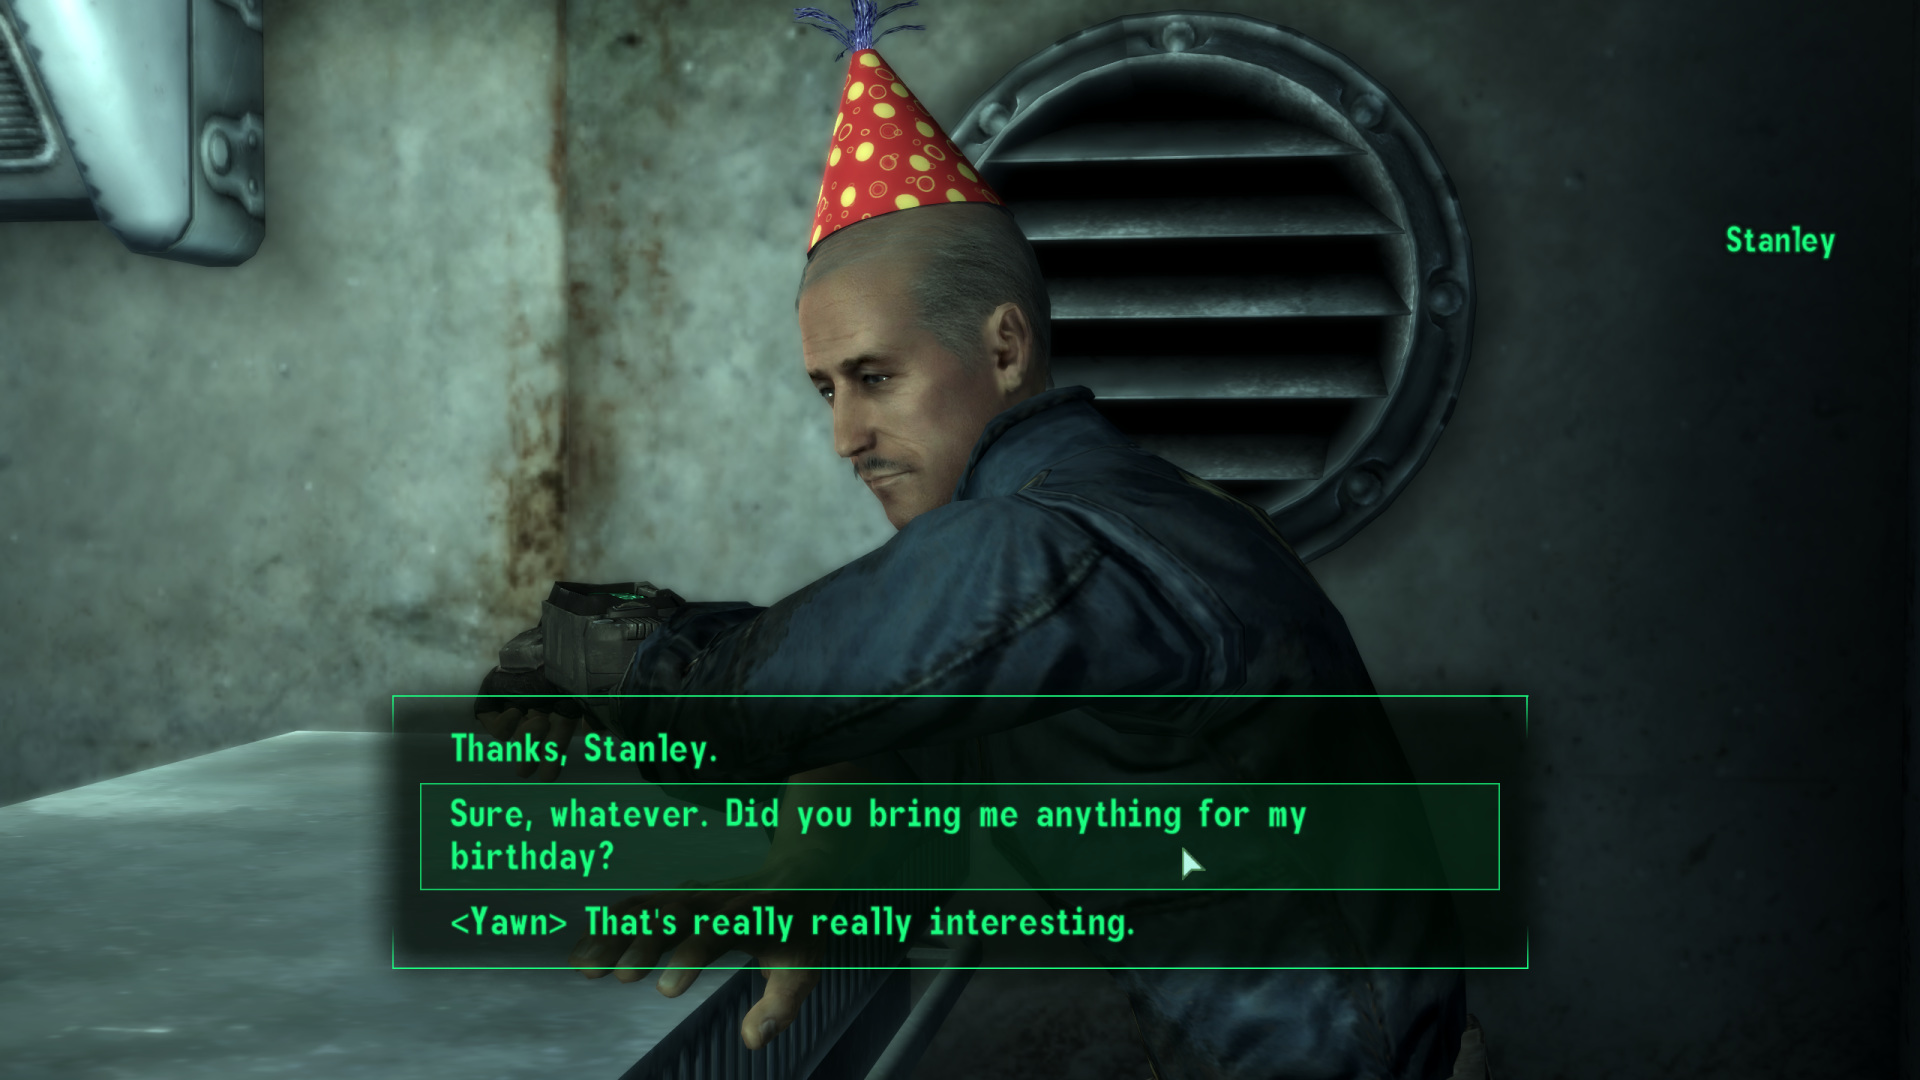
\includegraphics[width=0.6\textwidth]{images/fallout3}
\caption{Kadr z gry Fallout 3 przedstawiający przykładowy dialog}
\end{figure}

\href{https://assetstore.unity.com/packages/tools/utilities/dialogue-editor-168329}{Dialogue Editor} autorstwa Grasshop Dev jest prostym narzędziem pozwalającym na szybkie dodawanie i modyfikację dialogów.
Zawiera zestaw elementów ułatwiających wdrożenie systemu do projektu oraz udostępnia struktury danych wykorzystywanych do tworzenia interfejsu użytkownika.
Podczas rozmowy z postaciami niezależnymi gracz będzie mógł pozyskać informację o geografii świata, możliwych zagrożeniach oraz zadaniach do wykonania. 
Podobne systemy występują w grach takich jak Pillars of Eternity oraz w grach z serii Mass Effect.


\chapter{Sztuczna inteligencja przeciwników}

W przypadku implementacji mechanizmów sztucznej inteligencji przeciwników będziemy się inspirować trybami kampanii w grach Warcraft III oraz Starcraft II. 
Na mapie będą rozsiane punkty, w których będą pojawiać się przeciwnicy. 
Tak długo, jak drużyna gracza jest poza zasięgiem, wrogowie pozostają nieaktywni. 
Aktywni przeciwnicy zachowują się zgodnie z ich archetypem (klasą postaci) oraz pozostają aktywni tak długo, jak drużyna gracza jest w zasięgu. 
Zdezaktywowani przeciwnicy wracają do swojego oryginalnego stanu. Gracz będzie napotykał tego typu obozowiska przede wszystkim w trakcie eksploracji świata. 
Innym planowanym przykładem implementacji sztucznej inteligencji przeciwników jest model, w którym jednostki wroga poruszają się z punktu początkowego w stronę bazy gracza. 
Jeśli podczas swojej podróży napotkają drużynę gracza, wtedy niezwłocznie zmieniają swój cel ataku.
Będziemy wyróżniać trzy archetypy jednostek w zależności od sposobu walki (bliski zasięg, średni zasięg, daleki zasięg). 
Postacie walczące na bliski zasięg mają na celu podejście w stronę najbliższego przeciwnika i wykonać atak. 
Jednostki średnio zasięgowe w momencie, w którym najbliższy przeciwnik jest odpowiednio daleko, wykonują atak dystansowy, 
w przeciwnym wypadku zachowują się tak jak jednostki walczące w zwarciu. 
Postacie  dalekodystansowe dokonują ataków dystansowych w kierunku najbliższego przeciwnika, natomiast uciekają, gdy ten podejdzie zbyt blisko.

Przeciwnicy są kontrolowani poprzez jeden obiekt przydzielający cele każdemu przypisanemu wrogowi. W normalnym trybie wrogowie poruszają się w sposób losowy
w obrębie wyznaczonej przestrzeni (biały okrąg). Kiedy przyjazne jednostki znajdą się w wystarczającej odległości (czerwony okrąg), przeciwnicy obiorą sobie za cel jedną z nich.
Po opuszczeniu przez drużynę gracza wyznaczonego obszaru (żółty okrąg) wrogowie wracają do poruszania się w sposób losowy w obrębie białego okręgu.

Nawigacja przeciwników została zrealizowana poprzez wbudowany w silnik Unity system NavMesh. Pozwala nam on na łatwe wyznaczenie powierzchni, po której mogą poruszać
się postacie niekontrolowane przez gracza oraz realizuję zadanie wyznaczania ścieżki dla tych postaci.

\begin{figure}[h]
\centering
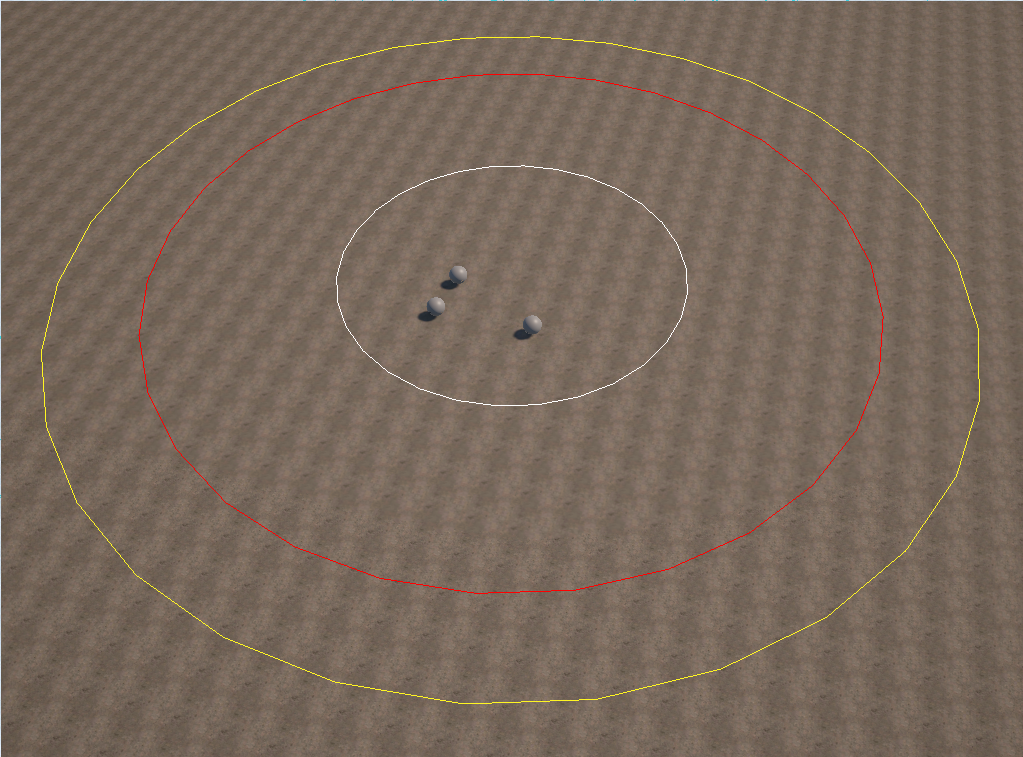
\includegraphics[width=0.6\textwidth]{images/ai}
\caption{Obraz przedstawia zasięgi odpowiednich regionów.}
\end{figure}

\chapter{Widzenie przez ściany}

Do umiejętności wykorzystywanych przez gracza będzie należeć zdolność widzenia przeciwników oraz innych istotnych obiektów przez przeszkody.
Gracz po wciśnięciu przycisku przez krótki okres będzie w stanie zobaczyć sylwetki przeciwników znajdującymi się w jego polu widzenia.
Grafika przedstawia rozwiązanie zawarte w grze Dead by Daylight. Markery nie poruszają się za celem lecz pojawiają się i pozostają w tym samym miejscu przez czas trwania animacji.

\begin{figure}[h]
\centering
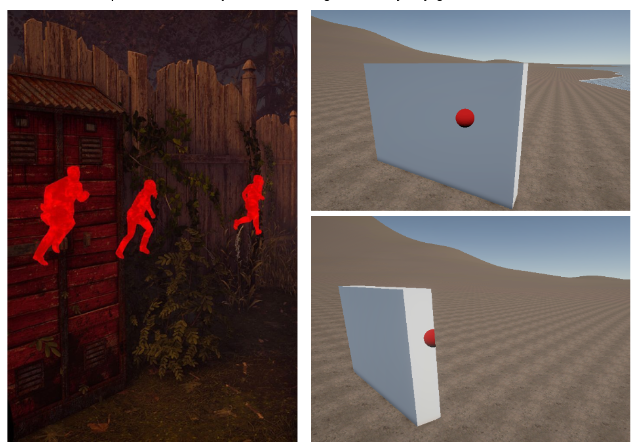
\includegraphics[width=0.6\textwidth]{images/shader}
\caption{Po lewej stronie przykład z gry Dead by Daylight. Po prawej zachowanie shadera w przypadku przysłanianiu markera przez przeszkody.}
\end{figure}

Efekt został osiągnięty poprzez zmodyfikowanie potoku renderowania w taki sposób, że w zależności od wartości w buforze głębi jest wykorzystywany inny shader.
W tym przypadku, jeżeli sfera jest przysłonięta przez ścianę jest ona narysowana w przeciwnym wypadku jest uruchamiany pusty shader.

Po naciśnięciu przycisku E następuje zagranie animacji opisanej wzorami $ w(t, offset) = 1.1 \times 2.1^{-\left(\frac{{\left(\sin(t) + 1 - 0.4 - \text{{offset}}\right)^2}}{{0.02}}\right)} $
oraz $ w(t, 0) - w(t, -0.2) + w(t, -1) - w(t, -1.2) $. Od podanych funkcji zależy przeźroczystość, jak i natężenie efektu Fresnela. 

\begin{figure}[h]
    \centering
    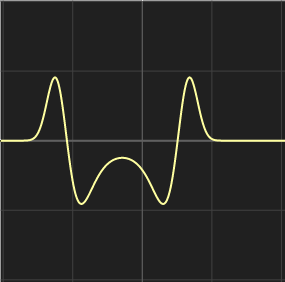
\includegraphics[width=0.25\textwidth]{images/g}
    \caption{Wykres przedstawiający funkcję opisującą zachowanie efektu Fresnela w animacji markera}
\end{figure}



\begin{lstlisting}[caption=Fragment shadera odpowiedzialny za animację]
fixed4 frag (v2f i) : SV_Target
{
  float t =  6.2 * _Progress - 0.6;
  fixed4 pattern = tex2D(_PatternTex, i.uv + _Speed *t);
  float fresnelInfluence = dot(i.worldPos, i.viewDir);
  float saturatedFresnel = saturate(1 - fresnelInfluence);

  float g = w(t, 0) - w(t, -0.2) + w(t, -1) - w(t, -1.2);
  float4 color = pow(saturatedFresnel, g * _FresnelPow) * (_Color * _ColorIntensity) * pattern;
  color.a *= dot(i.worldPos, i.viewDir);
  return color;
}
\end{lstlisting}

\chapter{Badania}\label{chap:research}

\chapter{Podsumowanie}\label{chap:summary}

% Bibliografia, ignorujemy overfull box, bo są długie URL
\hfuzz=50pt
\printbibliography[title=\bibliographyname]
\addcontentsline{toc}{chapter}{\bibliographyname}
\hfuzz=0pt

% Wykaz rysunków
\listoffigures
\addcontentsline{toc}{chapter}{\listfigurename}

% Wykaz tabel
\listoftables
\addcontentsline{toc}{chapter}{\listtablename}

\end{document}
